\documentclass[letterpaper, 10 pt, conference]{ieeeconf}

\IEEEoverridecommandlockouts
\overrideIEEEmargins              

\usepackage{cite}
\usepackage[pdftex]{graphicx}
\graphicspath{pictures/}
\DeclareGraphicsExtensions{.pdf,.jpeg,.png,.eps}
\usepackage{epstopdf}
\usepackage[cmex10]{amsmath}
\usepackage[caption=false,font=footnotesize]{subfig}
\usepackage{dblfloatfix}
\usepackage{fixltx2e}
\usepackage{color}
\usepackage{verbatim}
%\usepackage{algorithm2e}
%%\usepackage{algorithmicx}
%\makeatletter
%\newcommand{\removelatexerror}{\let\@latex@error\@gobble}
%\makeatother

%\hyphenation{op-tical net-works semi-conduc-tor}

% paper title
% can use linebreaks \\ within to get better formatting as desired
\title{\LARGE \bf
Applied Robotics for Installation and Base Operations \\for Industrial Hygiene}

%(ARIBO-IH)
% paresh comment: I will let you decide, but i think the title below is more descriptive but don't
% 					know if it will hurt your chances in TePra selection

% paresh suggested title:

% Autonomous Robotics for Installation and Base Operations Industrial Hygiene (ARIBO-IH) using an Unmanned Ground Vehicle (UGV) via Web-based User Interface for Command and Control

% author names and affiliations
% use a multiple column layout for up to three different
% affiliations
\author{Christopher Korpela, Kenneth Chaney, and Pareshkumar Brahmbhatt
\thanks{Manuscript received December 1, 2014. This work was supported in part by the Tank Automotive Research Development and Engineering Center (TARDEC). The views and conclusions contained herein are those of the authors and should not be interpreted as necessarily representing the official policies or endorsements, either expressed or implied, of the U.S. Government or TARDEC.}
\thanks{C. Korpela is with the United States Military Academy at West Point, NY 10996 USA \tt\small{christopher.korpela{@}usma.edu}}
\thanks{K. Chaney is with Drexel University in the Department of Computer Engineering \tt\small{kpc49{@}drexel.edu}}
\thanks{P. Brahmbhatt is with the University of Nevada, Las Vegas in the Department of Mechanical Engineering \tt\small{brahmbha{@}unlv.nevada.edu}}}


\begin{document}

\maketitle
\thispagestyle{empty}
\pagestyle{empty}

%%%%%%%%%%%%%%%%%%%%%%%%%%%%%%%%%%%%%%%
% Abstract
\begin{abstract}
A framework is proposed for Industrial Hygiene inspection using a remotely-operated ground vehicle with multiple sensor payloads attached to it for detecting various hazardous gases and chemicals. A control scheme and a graphical user interface between the vehicle and operator is strictly mandated for tasks requiring remote inspection. By leveraging existing navigation and path planning algorithms, the system can autonomously patrol hazardous areas and relay all measurements taken back to the user. This paper presents recent validation testing results of the system and its sensors using the proposed industrial hygiene framework.
\end{abstract}


%%%%%%%%%%%%%%%%%%%%%%%%%%%%%%%%%%%%%%%
% Introduction
\section{Introduction}\label{sec:introduction}

Throughout the Army, Industrial Hygiene (IH) teams are responsible for inspection, environmental reconnaissance, and emergency response. Industrial hygiene is an integral part of installation force protection and is an important component of an installation’s toxic industrial chemical spill planned response. Current best practices for conducting the IH mission requires direct human exposure to these hazardous environments. Robotic systems offer the potential to remove humans from these dangerous situations while maintaining the reliability and accuracy of the response team. Applying robotic solutions to this domain also contribute to the Department of Defense (DoD) unmanned systems goals outlined in the Unmanned Systems Integrated Roadmap FY2011-2036 \cite{roadmap}. Furthermore, robotic IH solutions are a force multiplier because these systems can be sent into a hazardous environment, parked, and allowed to collect data autonomously. Additionally, using robotic platforms for the IH environment is faster and safer than equipping and decontaminating a human. Finally, if successful, this project has potential DoD-wide application. 

\subsection{Trends}

Aging stocks of munitions and newly developed systems are creating larger quantities of dangerous materials that require monitoring and potentially, emergency response. In the current austere fiscal environment, enlarging a trained, professional IH team is a significant challenge. It is desirable to reuse/re-purpose existing inventory and to improve efficiency where possible.  One way to accomplish this goal is to automate tasks using technology such as robots and networked systems. This automation can allow a smaller team of trained personnel to effectively manage a large group of tasks.

\begin{figure}
	\centering
	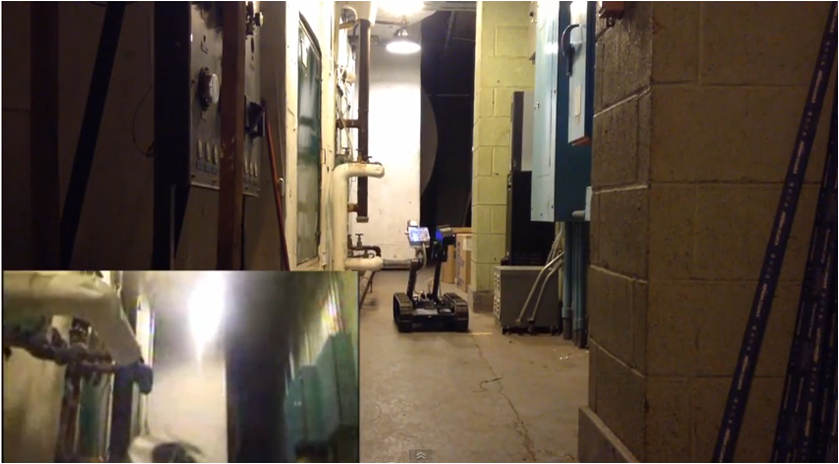
\includegraphics[width=0.48\textwidth]{./pictures/concept}
	\caption{ARIBO-IH prototype vehicle inspecting a gas leak in a notional hazardous site.}
	\label{fig:concept}
\end{figure}

\subsection{Problems}

An Industrial Hygiene mission is to reduce soldier and employee exposure to environmental factors and stresses including:  chemical (e.g., liquid, particulate dust, fumes, mist, vapor and gas), physical (e.g., electromagnetic radiation, temperature, ambient pressure, noise, vibration and ionizing radiation), and biological (e.g., agents of infectious diseases, insects, mites, molds, yeasts, fungi, bacteria and viruses) elements. The majority of hazards come from industrial processes on Army installations. Army industrial hygiene personnel are at risk from exposure to these hazardous environments in the conduct of their duties. Additionally, rapidly equipping human teams for response to incidents and post-action decontamination pose difficult challenges.  

\subsection{Benefits}

Through the use of robotic-enabled ground vehicles in a structured, controlled environment, the ARIBO-IH pilot will increase researchers’, manufacturers’, and users’ understanding and familiarity of these systems in real-world operational scenarios. The ARIBO-IH pilot safely provides the service of IH inspections, removing the human IH professional from a potentially hazardous situation while reducing cost. Additionally, the project will facilitate the design, standardization, deployment, and supervision of the resulting ARIBO-IH inspection robots. Finally, by using United States Military Academy (USMA) cadets as researchers, they are exposed to Army technologies and systems at the beginning of their careers.  The benefits of generating officers with technological backgrounds in robotics systems is paramount to achieving the DoD’s long term unmanned systems goals.

\subsection{Example Uses}
The robotic systems developed under this project could be employed in a number of situations to include:
\begin{itemize}
	\item Environmental reconnaissance in routine industrial hygiene tasks and emergency response
	\item Weather station at the emission source
	\item Ventilation duct inspection
	\item Investigate suspected terrorist devices
	\item Site abatement or mitigation projects
\end{itemize}

This paper presents a solution to the industrial hygiene problem using a small ground vehicle equipped with a sensor package. A control scheme for the system (Fig.~\ref{fig:concept} is implemented to allow for unattended operation in a known environment. Sec.~\ref{sec:model} details the kinematic and dynamic model for the system. The hardware and software components are found in Sec. \ref{sec:hardware}. Section~\ref{sec:results} presents validation results and sensor testing.

%%%%%%%%%%%%%%%%%%%%%%%%%%%%%%%%%%%%%%%
%Section: Hardware
\section{Chassis Design}\label{sec:chassis}

The iRobot PackBot is a fielded small robot used primarily for bomb disposal. The design is ``semi-modular'' where payloads can be installed to the base chassis, but they can only be installed in specific configurations, and when the software is properly configured. The integration of new payloads is often difficult and expensive. The vehicle uses military BB-2590 Li-Ion rechargeable batteries. While they have been widely deployed to both Iraq and Afghanistan, the Packbot is very expensive to purchase and maintain and overall reliability has been a challenge. There are two different generations: the obsolete 500 version and the current production 510 version. Many parts are interchangeable between the two models. The U.S. Army has discontinued the Packbot and no longer supports it as a program of record.

\begin{figure}
	\centering
	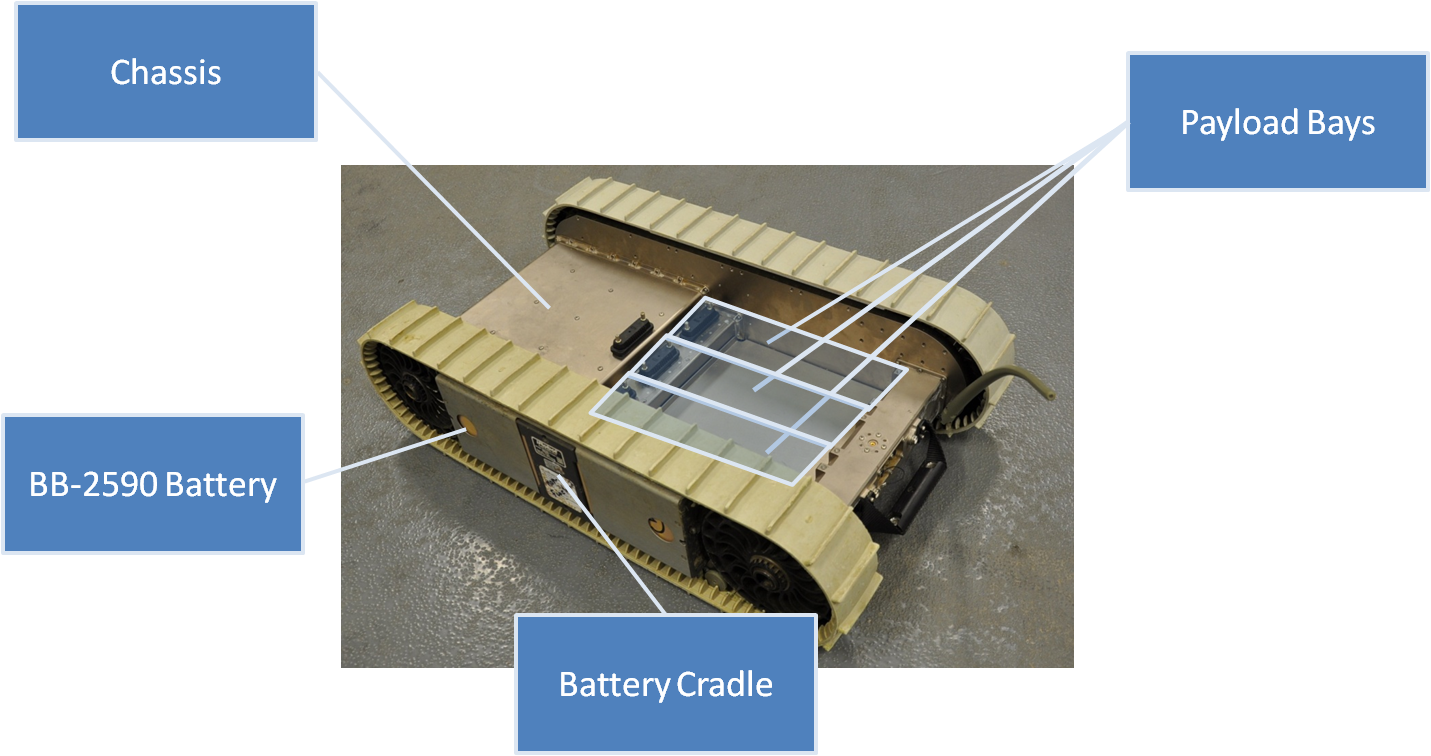
\includegraphics[width=0.48\textwidth]{./pictures/packbot.png}
	\caption{Anatomy of the Packbot.}
	\label{fig:packbot}
\end{figure}

With a large inventory of unused and unsupported robots, the RS-JPO (Robotic Systems Joint Program Office) funded a 12 month effort to implement IOP (Interoperability Profile V2, using JAUS which is the Joint Architecture for Unmanned Systems). Creating a kit design for retrofitting all fielded PackBots would reduce costs of maintaining the aged fleet. The standardized version of the PackBot makes a good research platform for a number of reasons:
\begin{itemize}
	\item Open architecture
	\item Design is completely government-owned
	\item Designed for IOP V1 compliance
	\item Cost relatively low
\end{itemize}
The research platform became known as GVR-Bot (Ground Vehicle Robotics is a branch of TARDEC). It changed the radio frequency to 2.4 GHz so it could easily connect over standard existing wireless Internet protocols. All of the internal electronics of the robot were replaced with new motherboards, interface boards, and motor controllers. Bootloaders were added to the internal control boards (allowing flashing of all the software without disassembling the robot). See Fig. \ref{fig:pcb} for an example circuit board.

\begin{figure}
	\centering
	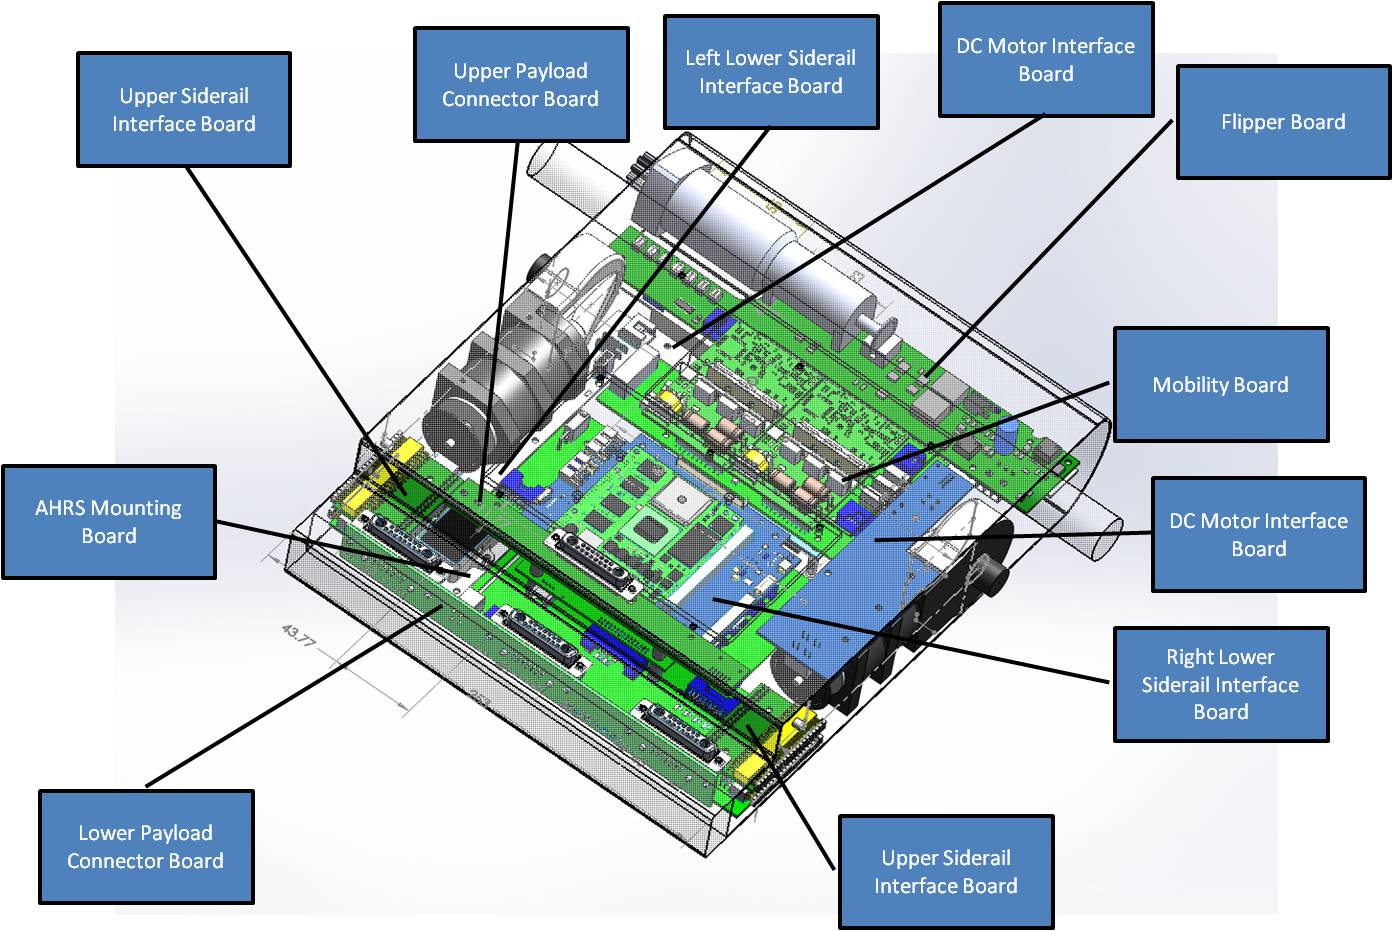
\includegraphics[width=0.48\textwidth]{./pictures/pcb.jpg}
	\caption{Front assembly interface board.}
	\label{fig:pcb}
\end{figure}


%%%%%%%%%%%%%%%%%%%%%%%%%%%%%%%%%%%%%%%
%Section: User Interface
\section{User Interface Software Suite}\label{sec:ui}

A standardized graphical user interface (GUI)\footnote{GUI is synonymous with Operator Control Unit (OCU).} was developed to be robust, intuitively usable by anyone, and serve as an all-in-one software suite (Fig. \ref{fig:gui_flow}) for servicing inputs and outputs via Robot Operating System (ROS) which acts as the backend of the GUI. The GUI frontend seen by the user is responsible for relaying environmental sensor and navigation data. The GUI software backend is standardized for use on any ground robot that is able to traverse through a 3 degree of freedom (DOF) work space ($x$,$y$,$\theta$) using an under-actuated controller. The user is able to control the robot's movement with a single virtual joystick controlling forward motion and turning. A wrapper is written to translate the joystick commands to actual motor commands. A second virtual joystick is available and dedicated to manipulating the camera viewpoint towards regions of interest in real time. This joystick allows the user to control a pan-tilt unit attached to the camera base. The camera feed and joystick bandwidth is automatically adjusted and delegated based on the bandwidth that is available at a particular instance between the robotic platform and the control unit. The GUI will alert the user if any bandwidth limits have been reached and will attempt to provide the user with the most up-to-date sensor and video data to allow the user to make the most informed decision possible in a given situation. Bandwidth concerns have a real impact upon mobile safety applications and must be taken into account; \cite{erikson2013} goes into further detail about how mobile constraints can alter the user interface and backend.

\begin{figure}
	\centering
	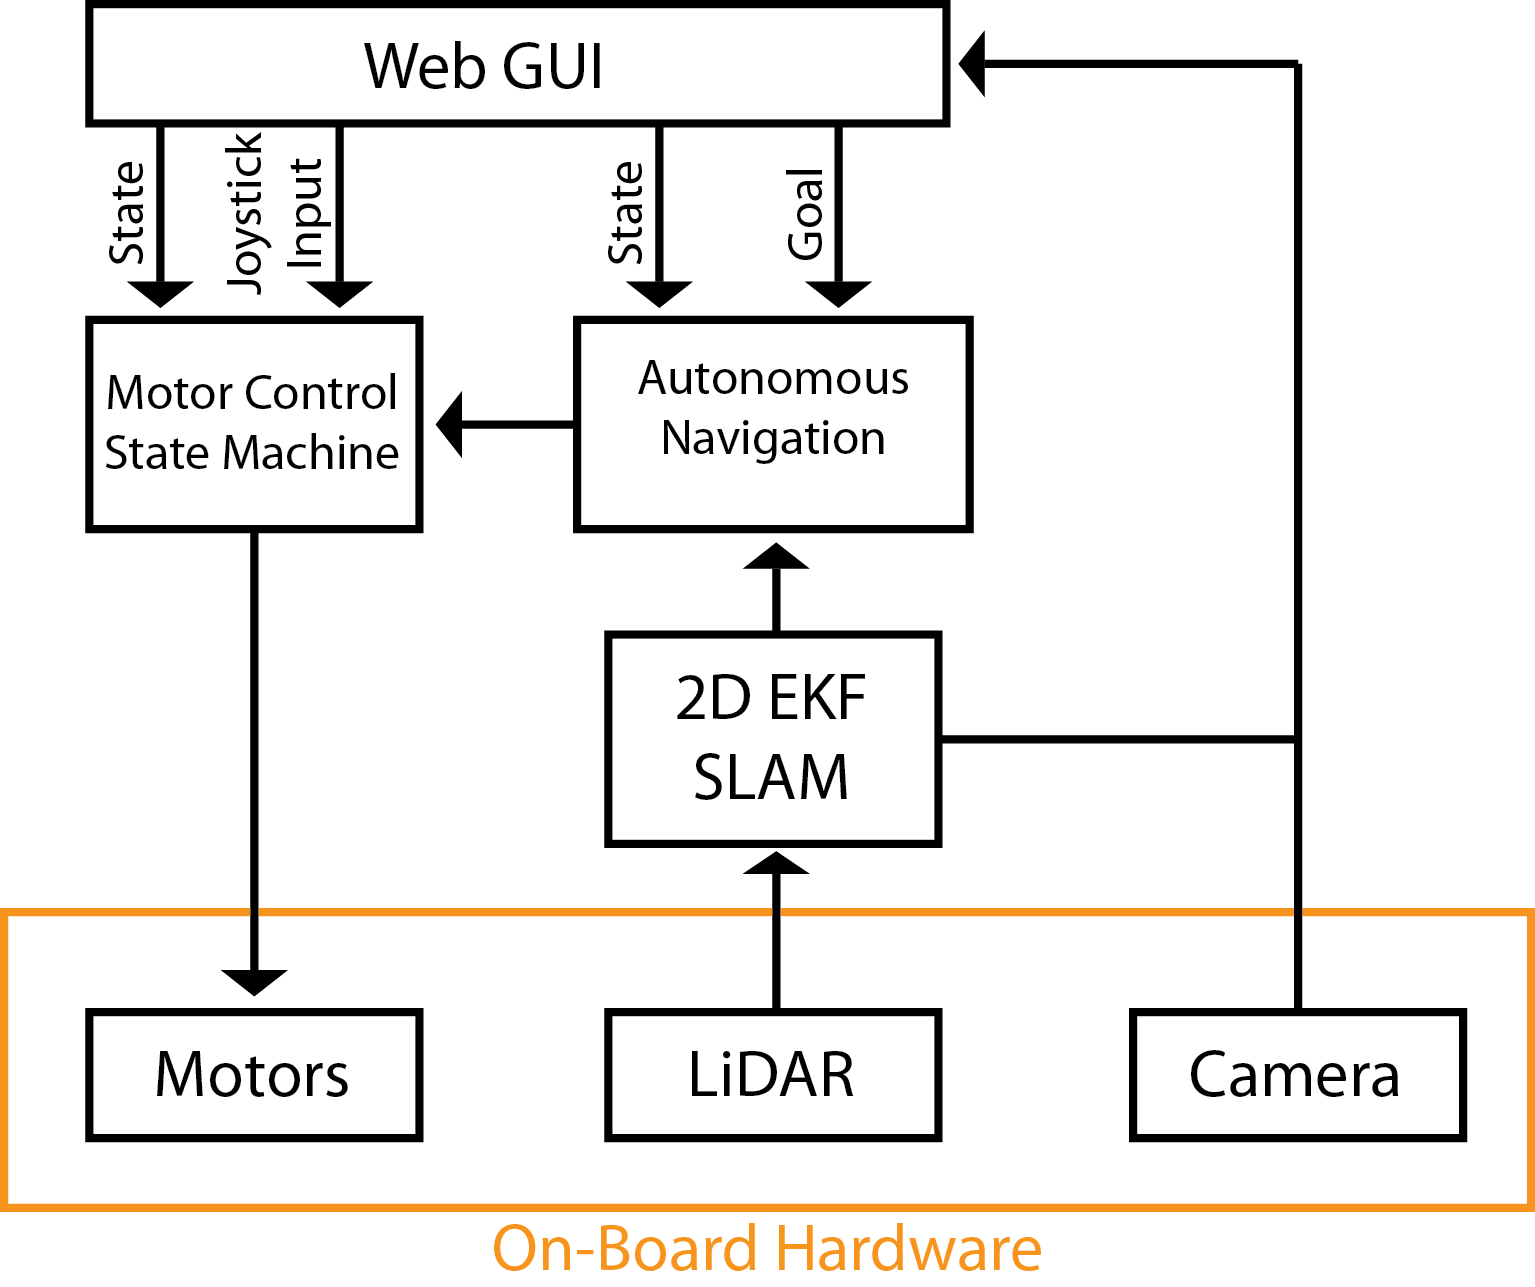
\includegraphics[width=0.48\textwidth]{pictures/Korpela_GUI.png}
	\caption{System flow of individual robot interface.}
	\label{fig:gui_flow}
\end{figure}

%To use this GUI for other ground robot platforms, all that would need to be developed is the wrapper code that translates the joystick into movement, assuming a different robot platform will have a different language coded onto its on-board system or motor controller. 

%While the control unit can be anywhere in the world, thus allowing the robot user to operate it through the internet or cloud service, there is better overall performance as well as lower latency in video stream, sensor data, and joystick data when the control unit is within the same compound as the robot. In ideal conditions, the user would be able to see and respond to any obstacle that is close by within low response time deltas, however under most conditions this isn't possible nor reasonable to expect. Low level obstacle avoidance function aids with basic navigation and reduces the probability of a crash that may be unforeseen by the user. The risk of the robot crashing into an obstacle cannot be completely mitigated because of several factors, but a few are real world delays in the data stream, loss of user's focus, lapses in data due to packet loss, the camera view is facing away from the obstacle, and connection loss.

%Another feature that has been built into the GUI is controlling based on way points instead of direct control over the robot. This allows for the user to click on the map to command the robot to navigate to the destination if possible. A 2D map is generated using SLAM from a LIDAR mounted on the robot--only differentials in the map are sent over the network. So while the initial connection may be slow, the delay during use is reasonalble. The 2D point that the user inputs is then fed into the navigation stack to attempt to reach the end goal. A third mode that the robot can be put into is pure autonomous navigation where the user can view what the robot is doing but won't have any control over the robot. The controller's multiple functionality allows for the user to pick the most appropriate mode of operation for a particular point in time, or to help the robot if it ever gets stuck. This is an important consideration when developing a GUI that is meant for long term industrial use, as all robots will eventually encounter something that they don't know how to deal with. 

\subsection{Navigation Modes}

As previously mentioned, the GUI allows the user to utilize two joysticks with one being for robot motion, and the other for camera pan-tilt motion; this two joystick scheme constitutes the first control mode. The GUI is designed to feature additional control modes. The control modes change the level of autonomy the robot exhibits during its mission. This feature, of course, requires for the different control modes to be hard-coded into the robot to ensure full functionality, both in terms of autonomous motion and safety of equipment in the facility being traversed. The change in control modes helps reduce the probability of mission failure or loss of robot if the control unit loses connection to the robot. The modes also change the level of involvement of the user in navigation duties, thus allowing the user to focus on higher level duties such as finding sources of contamination. This reduction of mental fatigue on the user helps increase missions success. All navigation modes utilize the GUI built-in features of map updating when differentials are found, obstacle proximity alerts, and environmental sensor warnings. 

% or thorough sterilization of the robot's local environment
%The second navigation mode provided through the GUI lets the user move the robot via way point navigation, which is done through a 2-Dimensional (2-D) interactive map of the compound that is provided to both robot and control unit prior to start of the mission. The robot is given way point locations to reach on the interactive map by the user during the start of its mission to alleviate future bandwidth needs that may arise as the mission progresses, and as bandwidth becomes restricted with increased distance from the control unit. These way points are generated by the interactive map feature after translating user input given via a mouse click-action on the 2-D map. If, for any reason, the robot is incapable of navigating to a way point it sends a warning message to the user indicating that autonomy has been reduced, and the robot has reverted back to control mode 1. The user can then use 2 joysticks to manually  maneuver the robot further into the compound or return it to the start point. After a predetermined amount of time, with no user input in control mode 1, the robot elevates autonomy and reverses course to return to the mission's start position using the way points taken to arrive at its current position. 

The second navigation mode allows for full autonomous exploration of the environment regardless of having any \emph{apriori} knowledge of the environment or not having a map. The robot uses LIDAR-based SLAM-EKF \cite{weingarten2005ekf, castellanos2007robocentric} to generate a map if none exists already. The map data is held in the on-board PC of the robot and can be transmitted on demand or streamed live. All navigation and obstacle avoidance actions are recorded on the full 3-D map, as metadata, that is generated as the robot progresses through the environment. Video data can also be toggled on if the user desires to visually inspect mission progress. By default, in order to reduce bandwidth saturation, map data is not transmitted to let mission critical sensor data take transmission priority.  A fail-safe feature sends a warning message to the user to indicate that the robot has reverted back to Mode 1 for manual navigation. This only occurs if the robot is unable to continue through the environment or has encountered a navigational error in its on-board programming. If the user takes no action or the connection has been lost, the robot again elevates autonomy to its original setting to reverse course and return to the mission start position. 

\subsection{HTML Interface}

The desire to create a web-based control application has been explored since the inception of the Internet \cite{goldberg2002beyond}. The GUI is a web application that has all the mentioned features to be toggled on or off through a settings window which is separate from the main robot interaction window in order to reduce the clutter the user sees while performing a mission (Fig. \ref{fig:gui_screenshot}). This will reduce the likelihood that the user will mistakenly click or press the wrong button during mission critical moments. The aforementioned navigation modes can be toggled on-the-fly by the user and are accessible directly from the main robot interaction window. The GUI frontend itself is based on Robot Web Tools \cite{webtools,lee2012web} which is a set of modules that help create web-based robot control applications. It allows ROS software package messages and topics to be accessible through a web interface that is constructed using HTML5 and Javascript via a wrapper called \textit{rosjs} \cite{osentoski2011robots}. The GUI is essentially a web accessible overlay that allows the user to send and receive data across a connection between a ROS server, the control unit, and its corresponding ROS client, the robot. The advantage of using HTML5 is its cross-platform compatibility allowing the web application to be used by PCs, tablets, and smart phones \cite{hilton2014lightweight}. On the ROS client, the robot computer runs a \textit{roscore} node that uses a package called \textit{rosbridge} which allows socket-based access to ROS through Javascript \cite{crick2011rosbridge}.

\begin{figure}
	\centering
	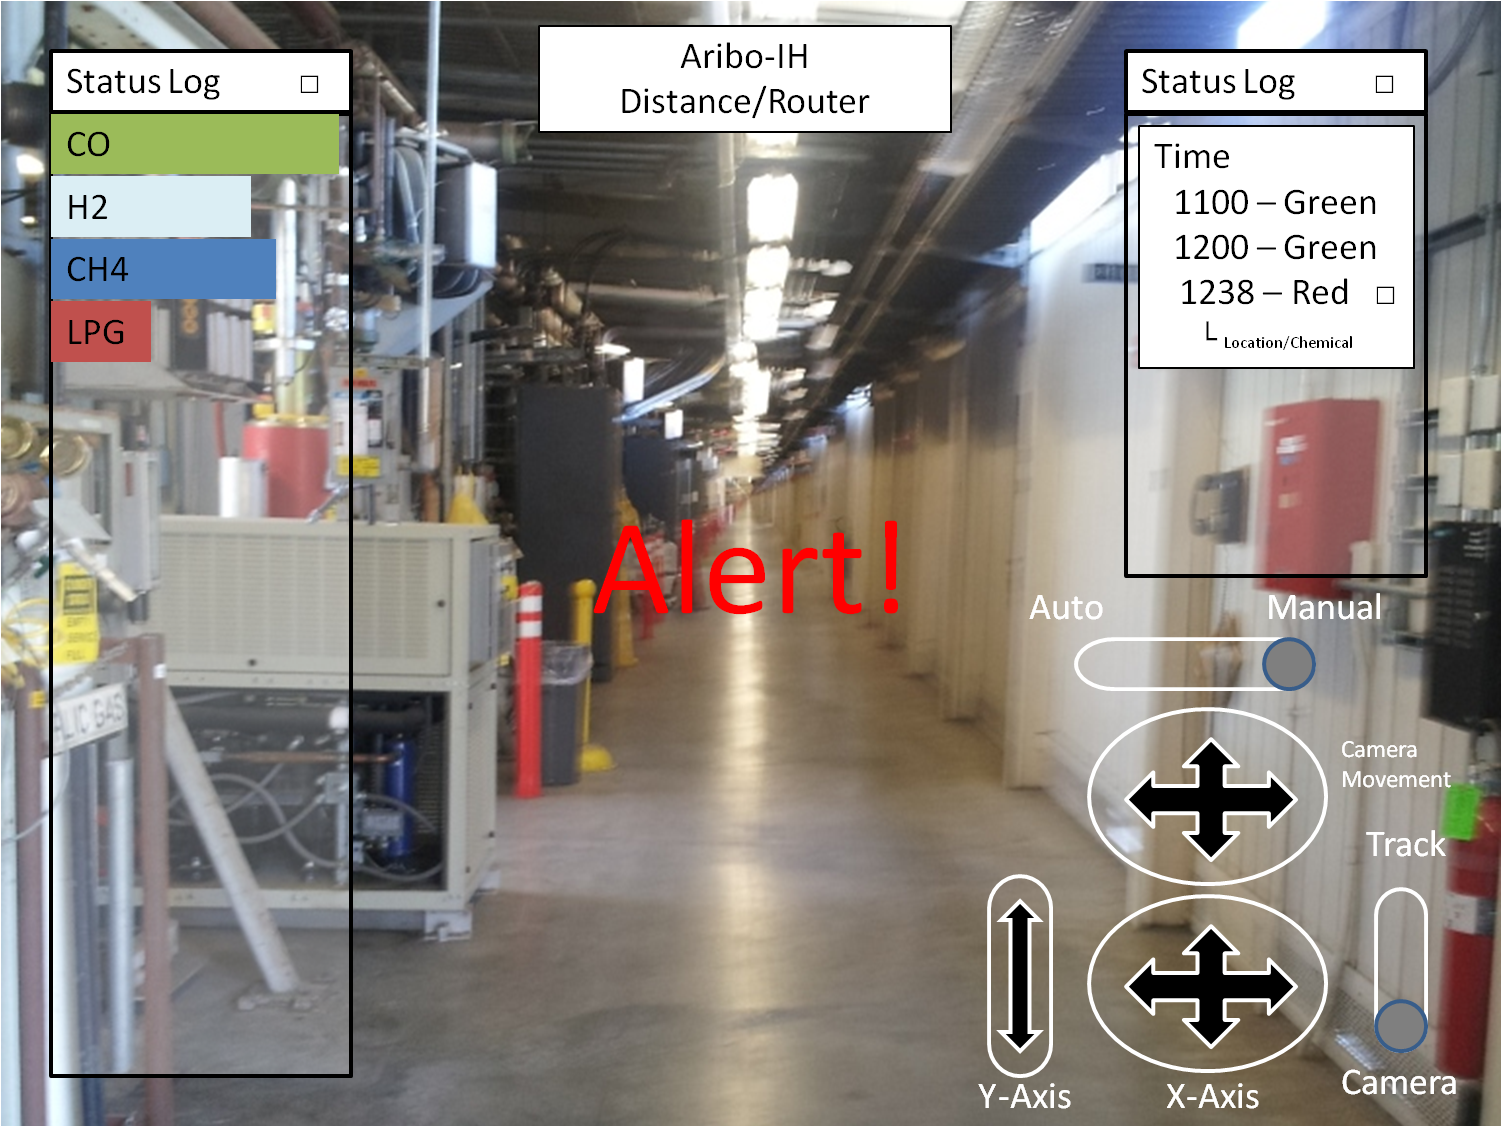
\includegraphics[width=0.48\textwidth]{pictures/gui-slac.png}
	\caption{Screenshot of the developed web-based GUI allowing for view of the camera and 2-D map.}
	\label{fig:gui_screenshot}
\end{figure}


%%%%%%%%%%%%%%%%%%%%%%%%%%%%%%%%%%%%%%%
%Section: Recharge
\section{Recharging}\label{sec:recharging}



%%%%%%%%%%%%%%%%%%%%%%%%%%%%%%%%%%%%%%%
%Section: Valve turning
%\input{content/valve_turning}

%%%%%%%%%%%%%%%%%%%%%%%%%%%%%%%%%%%%%%%
%Section: Valve
%\input{content/valve_features}
%\input{content/valve_detection}

%%%%%%%%%%%%%%%%%%%%%%%%%%%%%%%%%%%%%%%
%Section: Model
%\section{Modeling}\label{sec:model}
%The rigid body dynamics of rotorcraft are well understood \cite{Hoffmann2007}, \cite{Mahoney2012}. 
Much of the previous work in quadrotor control assumes the geometric center and quadrotor center of mass are coincident. With the introduction of two manipulators used for valve turning, the center of mass shifts and the inertia properties change based on arm joint angles and environmental contact forces and torques.

\begin{figure}
	\centering
	\includegraphics[width=0.4\textwidth]{./pictures/MMUAS}
	\caption{Coordinate System (links expanded for clarity). 4 DOFs are shown for each arm to indicate a future arm design.}
	\label{fig:ref-frame}
\end{figure}

\subsection{Aircraft-Arm Kinematics}
%A generalized 6-DOF vehicle model is proposed. 
The coordinate system for the aircraft-arm system is shown in Fig.~\ref{fig:ref-frame}.
%The world inertial frame $W$ is fixed and the body reference frame $B$ is placed at the vehicle center of mass as shown in Fig.~\ref{fig:ref-frame}. 
The position and orientation of the body frame %with respect to the inertial reference frame 
can be expressed in standard form as $p_b = [x \; y \; z]^T$ and $\phi_b = [\psi \; \theta \; \varphi]^T$ where the frames are right-handed with $Z$ pointed upward. Attitude is denoted by the yaw-pitch-roll Euler angles in the body frame ($Z\,Y\,X$). %The inertial frame is rotated by $R_b \in SO(3)$ to provide the orientation of the body frame.

%\begin{equation}
%	R_b(\phi_b) =
%	\begin{bmatrix}
%		c_{\psi}c_{\theta} & c_{\psi}s_{\theta}s_{\varphi}-s_{\psi}c_{\varphi}  & c_{\psi}s_{\theta}c_{\varphi}+s_{\psi}s_{\varphi} \\
%		s_{\psi}c_{\theta} & s_{\psi}s_{\theta}s_{\varphi}+c_{\psi}c_{\varphi} & s_{\psi}s_{\theta}c_{\varphi}-c_{\psi}s_{\varphi} \\
%		-s_{\theta}             & c_{\theta}s_{\varphi}                                              & c_{\theta}c_{\varphi} \\
%	\end{bmatrix}
%\end{equation}

The manipulators (noted as arms A and B with links $L_i$) are symmetrical and attached below the center of gravity of the quadrotor frame and equally offset from the vehicle's geometric center. Forward kinematics for the two serial chain manipulators are derived using Denavit-Hartenberg (DH) parameters as shown in Table~\ref{tab:DHParameters}. Parameters $\theta$, $d$, $a$, and $\alpha$ are in standard DH convention and  $q_i$ for $i = 1$ to $n$ are joint variables for the arm. The direct kinematics function relating the quadrotor body to the end-effector frame, $p_e$, is:

\begin{equation}
	p_e = p_b + R_bp^b_{eb}
\end{equation}
where $p^b_{eb}$ is the position of the end-effector with respect to the body frame. A similar analysis is performed in \cite{Arleo2013}.

\begin{table}
	\renewcommand{\arraystretch}{1.3}
	\caption{Denavit-Hartenberg Parameters for Manipulator}
	\label{tab:DHParameters}
	\centering
	\begin{tabular}{|c||c|c|c|c|}
	\hline
	Link & $\theta$ & d & a & $\alpha$\\
	Number & (rad.) & (mm) & (mm) & (rad.)\\
	\hline
	\hline 
	1 & $q_1$ & 0   & $L_1$ & 0\\
	2 & $q_2$ & 0   & $L_2$ & 0\\
	\hline
	\end{tabular}
\end{table}

\subsection{Aircraft-Arm Dynamics}

The equations of motion for the center of mass of the geometric center of the generalized 6-DOF vehicle have the standard Newton-Euler form \cite{Bouabdallah2004}:

\begin{subequations}
	\begin{align}
	\vec{F} = m_Q\vec{\dot{v}}+\mathbf{\Omega} \times m_Q\vec{v} \\
\vec{\tau} = \mathbf{I}\dot{\mathbf{\Omega}}+\Omega \times \mathbf{I} \mathbf{\Omega}
	\end{align}
\end{subequations}
where $F$ represents the combination of propeller, aerodynamic, and gravitational forces with vehicle mass, $m_Q$, linear velocity, $v$, linear acceleration, $\dot{v}$, and rotational velocity, $\Omega$. Torque, $\tau$, is calculated from the inertia matrix, $I$, and the rotational velocity and acceleration, $\Omega$ and $\dot{\Omega}$ respectively. The torque and force produced from the quadrotor propellers have to be taken into account. The torque $\vec{\tau}^i$ has two components, one coming from the actual propeller drag $Q$, and the other due to the displacement of the propeller from the center of mass $\Delta\vec{\mathbf{o}}_{CM}^i(q_j)$. In an aerial manipulator system, the center of mass shifts as each joint ($q_j$) of the manipulator rotates and the torque becomes a nonlinear function of the manipulator joint angles:

\begin{subequations}
\begin{equation}\label{eq:QuadForce}
\vec{\boldsymbol{F}}_{q}(u)=\sum_{i=1}^{4}\vec{\mathbf{F}}(u)^i\\
\end{equation}
\begin{equation}\label{eq:QuadTorque}
\vec{\boldsymbol{\tau}}_{q}(u,q_j)=\sum_{i=1}^{4}\vec{\mathbf{Q}}(u)^i+\Delta\vec{\mathbf{o}}_{CM}^i(q_j) \times \vec{\mathbf{F}}(u)^i
\end{equation}
\end{subequations}

%In a simple scenario, when only a single joint (i.e. $q_2$) moves, the changing moment of inertia term resulting from arm movement can be calculated using the parallel axis theorem. Although simplified, this methodology is a realistic calculation of the moment of inertia where:
%\begin{equation}\label{eq:inertia}
%	\textbf{I}=\frac{m{D_2}^2}{12}+\frac{mD_2^2}{4}sin(q_2)^2
%\end{equation}
%with $q_2$ as the angle between the axis of rotation and link $D_2$. For the proposed valve turning scenario the applied arm torque onto the quadrotor body is:
%\begin{equation}\label{eq:torque}
%	\tau_{manip} = F_{link}D_2sin(\Theta)
%\end{equation}
%where $F_{link}$ is the link force experienced by the gripper of the manipulator and $D_2$ is the link distance. This torque is first applied to the 2nd joint, and is consequently applied to the quadrotor body.

%Given the dynamic model for both manipulator and the quadrotor body, a simplified arm model is utilized for the complete system. 
%Considering simplified dynamics and not accounting for various aerodynamic effects (i.e. blade flapping, ground effect, etc.) experienced during highly dynamic flying maneuvers, it is possible to emulate the aircraft behavior on a 6-DOF gantry system\cite{Korpela2014}. Most of the vehicle's critical motions occur around hover where small angle approximations can be used. Our previous results show that it is possible to emulate the problem of UAV control on a gantry testbed using similar control approaches. In this paper we pursue this path in order to verify and test UAV-like behavior when performing valve turning. %This fact justifies a simplified mathematical model.

%%%%%%%%%%%%%%%%%%%%%%%%%%%%%%%%%%%%%%%
%Section: Model
%\input{content/coupling}

%%%%%%%%%%%%%%%%%%%%%%%%%%%%%%%%%%%%%%%
%Section: Control
%\section{Control}\label{sec:control}

%\subsection{Attitude Control}

%Taking into account the dynamics of the system, a simplified Proportional controller for the corresponding attitude loop, and a Proportional-Integral controller for the position loop is proposed. Effectively, this transforms the proposed two stage cascade controller structure into a single PI-Derivative position controller. The proposed PI-D controller equation~(\ref{eq:ControlLaw}) implies that the control difference $\vec{e}$ is taken through the proportional and integration channels, while the derivative channel is connected directly to speed measurements of the quadrotor $\vec{v}_0$. Equations are written in vector form because they are applied to $x, y, z$ positions in 3D space.

%\begin{equation}\label{eq:ControlLaw}
%	\centering
%	\begin{aligned}
%	\vec{u}=K_P \vec{e} + K_I\int {\vec{e}}+ K_D \vec{v}_0 
%	\end{aligned}
%\end{equation}

%\begin{figure}[t]
%	\centering
%	\includegraphics[width=0.5\textwidth]{./pictures/simulation}
%	\caption{MM-UAV Control Structure}
%	\label{fig:MMUAVControlStructure}
%\end{figure}

%$K_P$, $K_I$, and $K_D$ are the PI-D control gains. Error vector $\vec{e}$ is the difference between the $x, y, z$ position data and the actual setpoint reference values, and $\vec{v}$ is the speed measurement. Due to the fact that the derivation channel (i.e. aircraft speed) is error sensitive, leading the control difference directly through can cause serious problems and possibly damage the aircraft. On the other hand, position data is much more reliable and can be used directly in the control loop. PI-D position control is implemented as a Python class, running at a 20 Hz refresh rate.

%\subsection{Feature Detection through Ellipsoid Tracking}

%Feature detection has been extensively used by rotorcraft to achieve hover for surveillance and localization \cite{Bourquardez2009}, \cite{Romero2006}. 

%\cite{Ahmadzadeh2013}

%\subsection{Visual Servoing and Position Control}

%\begin{figure}[b]
%	\centering
%	\includegraphics[width=0.5\textwidth]{./pictures/MMUAS_peg_in_hole}
%	\caption{Camera Reference Frame (camera in an exploded view for clarity)}
%	\label{fig:camera}
%\end{figure}

%Image Based Visual Servoing (IBVS) has been extensively used by rotorcraft to achieve hover for surveillance and localization \cite{Bourquardez2009}, \cite{Romero2006}. An \emph{eye-in-hand} system is used where the camera is attached to the end-effector. The camera frame relative to the end-effector frame is known \emph{a priori} as shown in Fig.~\ref{fig:camera}. The transformation between the image feature velocities, $\dot{s}$, and the joint velocities, $\dot{q}$, must be determined where:

%\begin{equation}
%	s=J(x,y,Z,q) \dot{q}
%\end{equation}
%The center location of the camera frame $(u,\;v)$ is projected into Cartesian coordinates where $C = (X_C, \; Y_C, \; Z_C)$ of the center of the hole. Using the center location, $d$ is calculated to determine the distance of the target hole to the camera.

%The control inputs consist of $x, \; y, \; z$ position and yaw $\psi$ orientation of the quadrotor, yaw joint $q_1$, pitch joint $q_2$, and roll joint $q_3$ of the end-effector. The total controllable degrees of freedom for the aircraft-arm system is seven. As the wrist is spherical with intersecting axes of rotation, the inverse kinematic calculations are greatly simplified to determine joint angles for a desired pose and orientation. The arm can be described as a series of transforms:

%\begin{equation}
%	T = A_{0T} = A_{01}A_{12}(q_1)A_{23}(q_2)A_{3T}(q_3)
%\end{equation}
%where $A_{01}$ is the fixed transform from the center of a quadrotor and $A_{3T}$ is the transform from the last joint of the arm ($q_3$) to the tool tip. $A_{AB}$ is the transform from joint A to joint B and is driven by the angle of joint $A(q_A)$. With the vehicle at a specified position and yaw orientation, the next step is to solve for the spherical wrist joints ($q_1, q_2, q_3$) using the method described in \cite{Tsai1985}. The first step in this process is to identify the transform that represents the combined joint rotations from the wrist to the target $(A_{3T})$ where:
%\begin{equation}
%	A_{3T} = A^{-1}_{3T}
%\end{equation}
%Next, $q_1, q_2$, and $q_3$ are calculated directly from $A_{3T}$ where:

%\begin{subequations}
%\begin{align}
%q_1 = atan2(A_{3T}[2,3],A_{3T}[1,3]) \\
%q_2 = atan2(\sqrt{(A_{3T}[1,3]^2+A_{3T}[2,3]^2},A_{3T}[3,3]) \\
%q_3 = atan2(A_{3T}[3,2],-A_{3T}[3,1])
%\end{align}
%\end{subequations}
%to generate the closed form solution for the joint angles.

%\subsection{Force Feedback}

An impedance control strategy is proposed to control the dynamic interaction between the manipulators and their environment. Impedance control enables contact between the manipulator and its environment while maintaining stability during the transition from free motion to interaction \cite{Hogan1984}. In a simplified manner, the manipulators can be seen as a mass-spring-damper system behaving like an impedance towards the environment. The controller applies prescribed interaction forces at the end effector which are calculated as:

\begin{equation}
 	F_{int}=K[X_0-X]
	\label{eq:eq7}
\end{equation}
where $F_{int}$ is the desired interaction force to be applied at the end effector, and $X_0-X$ is the position error and $K$ is a stiffness gain to map between position error and interaction force. $K$ can be thought of as a spring constant while $X_0-X$ can be thought of as the spring's compression. (\ref{eq:eq7}) can be rearranged to solve for a pseudo-goal position to command the end effector to, using the position controller that will impart the desired amount of force. To achieve this, we need to calculate the torques necessary to command each joint where:

\begin{equation}
	T_{act}=J^{\#T}F_{int}
	\label{eq:eq8}
\end{equation}
Combining \ref{eq:eq7} and \ref{eq:eq8}, we have:

\begin{equation}
	T_{act}=J^{\#T}K[X_0-X]
	\label{eq:eq9}
\end{equation}
to represent overall commanded joint torques.

%%%%%%%%%%%%%%%%%%%%%%%%%%%%%%%%%%%%%%%
%Section: Validation
%\section{System Validation and Results}\label{sec:validation}

To test and validate the valve turning framework, the system was implemented on a miniature gantry system. Dubbed Mini-SISTR, the gantry is modeled after the Systems Integrated Sensor Test Rig (SISTR) \cite{Korpela2014}. The experimental setup is shown in Fig. \ref{fig:gantry-quad}. The miniature gantry can traverse 0.35 m/s along each $x$, $y$, and $z$ axis. To provide yaw, pitch, and roll angles and velocities for the emulated aircraft, a 3-DOF gimbal is attached to the gantry z-axis. 

\begin{figure}
	\centering
	\includegraphics[width=0.45\textwidth]{./pictures/gantry.jpg}
	\caption{Mini-SISTR test and evaluation gantry rig.}
	\label{fig:gantry-quad}
\end{figure}

\subsection{Valve Turning Tests}

A series of valve turning experiments were performed for model verification. The valve is plastic and scaled to an actual industrial valve with an outer diameter of 15 $cm$. Fig. \ref{fig:valve-turn-test} shows a series of snapshots during a valve turning experiment. 

\begin{figure}[b]
	\centering
	{\subfloat[Detect valve using Hough transform. The aircraft-arm system aligns itself with valve.]{\includegraphics[width=0.35\textwidth]{pictures/shot1a.jpg}}
	\vfil
	\subfloat[Grab onto valve. The two arms articulate and grasp the valve until a desired joint torque is met. Note the orientation of the PVC pipe (left right).]{\includegraphics[width=0.35\textwidth]{pictures/shot2a.jpg}}
	\vfil
	\subfloat[Perform 1.57 radians turn. The yaw motion of the vehicle allows the valve to turn while the system is coupled. Note the new orientation of the PVC pipe (up down).]{\includegraphics[width=0.35\textwidth]{pictures/shot3a.jpg}}}
	\caption{Valve turning experiment while attached to the gantry test rig.}
	\label{fig:valve-turn-test}
\end{figure}

\subsection{Controller Performance}

Fig.~\ref{fig:plot1} shows the applied torques to the UAV yaw axis, right shoulder joint, right wrist joint, left shoulder joint, and left wrist joint of the two arms. When the arms make contact with the valve, the right and left shoulder joints experience the greatest applied torque throughout the turn. The wheel is rotated 1.57 radians in a clockwise direction with the quadrotor yaw torque shown in blue. The wheel is released at time stamp 25 sec. and then regrasped at time stamp 30 sec. The wheel is then rotated 1.57 radians in a counterclockwise direction. The applied torques by both shoulder and wrist joints provide a compliant and consist grasp during the valve rotation.

\begin{figure}
	\centering
      	{\subfloat[Quadrotor yaw torque and shoulder roll joint torques for both arms (Nm vs. time).]{\includegraphics[width=0.5\textwidth]{./pictures/shoulder.eps}}
	\vfil
      	\subfloat[Quadrotor yaw torque and wrist roll joint torques for both arms (Nm vs. time).]{\includegraphics[width=0.5\textwidth]{./pictures/wrist.eps}}}
	\caption{Applied torques during valve turning. The first grab and turn occurs between 10 and 25 seconds. The valve is released at time stamp 25 sec. and regrasped at time stamp 30 sec. for another rotation in the opposite direction.}
	\label{fig:plot1}
\end{figure}

%SISTR was developed as a hardware-in-the-loop test rig and designed to be used to evaluate obstacle detection sensors (LIDAR, computer vision, ultrasonic, ultra-wideband radar, millimeter wave radar, etc.), design sensor suites, and test collision avoidance algorithms.

%The miniature gantry can traverse 0.35 m/s along each $x$, $y$, and $z$ axis. To provide yaw, pitch, and roll angles and velocities for the emulated aircraft, a 3-DOF gimbal is attached to the gantry z-axis. Mini-SISTR can be tuned for almost any rotorcraft model in hover or near-hover modes. Models to account for ground-effect can also be incorporated to study perturbations and disturbances. For this particular analysis, the quadrotor model developed in Sec. \ref{sec:model} is implemented. The actual vehicle as described in Sec. \ref{sec:hardware} is 50 $cm$ in diameter and weighs 1.5 $kg$ where the gantry imitates the flight dynamics of this vehicle. 

%Using a recursive Newton-Euler algorithm and neglecting friction forces, one can derive generalized force/torque equations produced from each joint movement of the manipulators:

%\begin{equation}
%\sum_{j=0}^{n}[D_{ij}(\mathbf{q})\ddot{q}_j]+\sum_{k=0}^{n}\sum_{j=0}^{n}[C^i_{kj}(\mathbf{q})\dot{q}_k\dot{q}_j]+h_i(\mathbf{q})=\tau_i,0\leq i \leq n
%\label{eq:CompleteArmModel}
%\end{equation}
%with $D_{ij}$ as a generalized inertia tensor, $C^i_{kj}$ is the generalized Coriolis and Centrifugal force matrix and $h_i$ is a generalized gravity force. 

%Given that $\tau_0$ calculates forces produced on the aircraft body (i.e. $w=\tau_0$), Newton-Euler analysis provides the necessary tools to calculate static and dynamic disturbances acting on the rotorcraft. In a complete model, Newton-Euler equations for manipulator motion need to be provided with initial angular and linear speeds and accelerations. To simplify the overall problem, we make a reasonable assumption that the aircraft is in hover during manipulation. This assumption enables us to regard the initial linear and angular dynamics of the aircraft body as zero, thus effectively decoupling the dynamics.

%\subsection{Applied Torque Model}

%The 6-DOF miniature gantry utilizes a torque model to reproduce the reactions the aircraft undergoes when subjected to moments applied by the manipulator, interactions with the environment, or added load masses. The 3-axis gimbal provides yaw-pitch-roll position, velocity, torque, and impedance feedback and control. The applied torque is tuned according to the mass and inertial properties of the vehicle. A rotorcraft with a larger mass and inertia will be able to withstand larger pitch and roll moments compared to a vehicle with less mass and inertia. The basic assumption for the quadrotor in hover is that the thrust force and the force of gravity are equal:
%\begin{equation}
%\sum_{i=1}^{4}\vec{F}_i=m_Q\cdot \vec{g},
%\end{equation}
%where $\vec{q}$ represents the gravity acceleration vector. The quadrotor translates by tilting slightly in the desired direction. Therefore, for a small angle approximation, $x$ and $y$ coordinate dynamics can be derived. For clarity, we are showing only $x$ axis dynamics (i.e. force in the $x$ direction $F_x$ and respective acceleration $a_x$), produced from the quadrotor pitch angle $\Theta$. 
%\begin{equation}
%\begin{split}
%F_x =m\cdot g\,  \textup{sin}(\Theta) & \sim m_Q g \Theta\\
%a_x & \sim g\Theta
%\end{split}
%\end{equation}

%Because the aircraft interacts with the environment, the applied torques are fed into the simulated aircraft model. The attitude controller ultimately needs to compensate and correct these disturbances. Both static (constant torque applied by the manipulator mass) and dynamic (moving torques associated with articulation and environmental contact) are sensed by the attitude controller. This approach allows us to write a simple dynamic model for the emulation of quadrotor dynamics seen in Fig. \ref{fig:controller}.

%\begin{figure}
%	\centering
%	\includegraphics[width=0.5\textwidth]{./pictures/GantryAngleController.jpg}
%	\caption{Angle Attitude Controller (needs updating)}
%	\label{fig:controller}
%\end{figure}

%The disturbance force, $F_D$ is mapped from the applied torque, $\tau_D$, which contributes to the linear acceleration, $a_x$, of the vehicle base. $J$ is the inertial tensor for the 6-DOF aircraft. The linearized equation for $\tau_D \mapsto F_D$ mapping can be derived from the complete dynamic model of the arm in (\ref{eq:CompleteArmModel}). The acceleration resulting from the torque distance has the form:
%\begin{equation}
%	\centering
%	a_x = g\Theta + \frac{\tau_D \mapsto F_D }{J}
%\end{equation}
%Moments applied to the aircraft first introduce changes to angular positions and velocities which change the thrust vector. This altered thrust vector then causes a lateral translation in the vehicle. The torso joint positions adjust accordingly to emulate the pitching and rolling motions and the gantry provides the linear displacement in the $x$ and $y$ directions. Direct forces such as aerodynamic effects, propeller wash or ground effect, and wind gusts are not modeled. The forces and torques that do influence the vehicle pose are environmental contact through the end-effector, added load masses, and the mass and inertia of the manipulator itself.

%The second additive component to linear acceleration of the vehicle results from the projection of the gravity vector onto the $x$ or $y$ axis when the vehicle pitches or rolls. The angular position changes based on the linear velocity error and a proportional gain. As mentioned, the changing thrust vector due to a pitch or roll movement translates into a linear acceleration. 

%\subsection{Velocity Control Loop}

%The block diagram for the attitude controller is found in Fig. \ref{fig:controller}. 
%The reference velocity is set by the user through a joystick interface. This velocity is compared to the actual gantry velocity provided by a encoders on the gantry actuators. The error is fed into a PID controller which calculates the angular position required to translate the gantry and eliminate the error. The angle is projected onto the linear axis as acceleration through the gravity vector. The angular position of the aircraft changes in the same direction as the applied force. The measured torque, converted into a disturbance force and divided by the system mass, also contributes to the linear acceleration. An integrator converts acceleration into velocity which is sent to a gantry controller to actuate the gantry motors. Since the inertia properties are used to calculate the emulated UAV velocity, the controller can be tuned for almost any rotorcraft.


%%%%%%%%%%%%%%%%%%%%%%%%%%%%%%%%%%%%%%%
%Section: Results
\section{Sensor Testing and Results}\label{sec:results}

Since gas sensors are inherently inaccurate due to their manufacturing processes and biases, each sensor had to be calibrated by graphing the output of each sensor compared to the known gas in the testing environment. The testing environments consists of 1.0 liter sealed containers with the sensor inserted into one end and a septum for needles inserted in the other as illustrated in Fig. \ref{fig:sensor}. The 1.0 liter volume simplified the calculations in parts-per-million (ppm) and each gas was introduced to the environment via a syringe and needle.

\begin{figure}
	\centering
	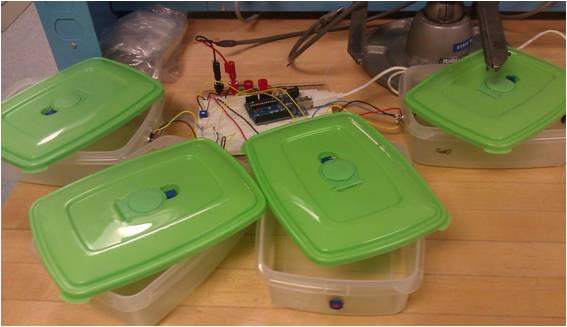
\includegraphics[width=0.48\textwidth]{./pictures/sensor.jpg}
	\caption{Testing environments (from left to right): MQ-4, MQ-6, MQ-7, and MQ-8 sensors.}
	\label{fig:sensor}
\end{figure}

By comparing the sensor output (x-axis) to the known concentration of gas in the testing environment (y-axis), a curve is formed, which can be best fit to an exponential curve by focusing the comparison on moderately to severely dangerous gas concentrations, which is approximately 2,000 to 10,000 ppm. The best fit equation for the most accurate test is used in software to correct the sensor output to the most accurate output for transmission to the operator through the GUI. Figs. \ref{fig:methanetoxic}-\ref{fig:hydrogen} display the graph for the MQ-4 (Methane) sensor along with the graphs for MQ-6 (Liquefied Petroleum Gas), MQ-7 (Carbon Monoxide), and MQ-8 (Hydrogen) sensors.

\begin{table}
	\centering
	\begin{tabular}{|c||c|}
		\hline
		Test & \(R^2\) \\ \hline \hline
		Methane Toxicity & 0.996 \\ \hline
		Methane Test & 0.994 \\ \hline
		LPG Test & 0.999 \\ \hline
		CO Test & 0.998 \\ \hline
		Hydrogen Test & 0.969 \\ \hline
	\end{tabular}
	\caption{\(R^2\) values associated with fit curves in Figs. \ref{fig:methanetoxic}-\ref{fig:hydrogen}}
\end{table}

\begin{figure}
	\centering
	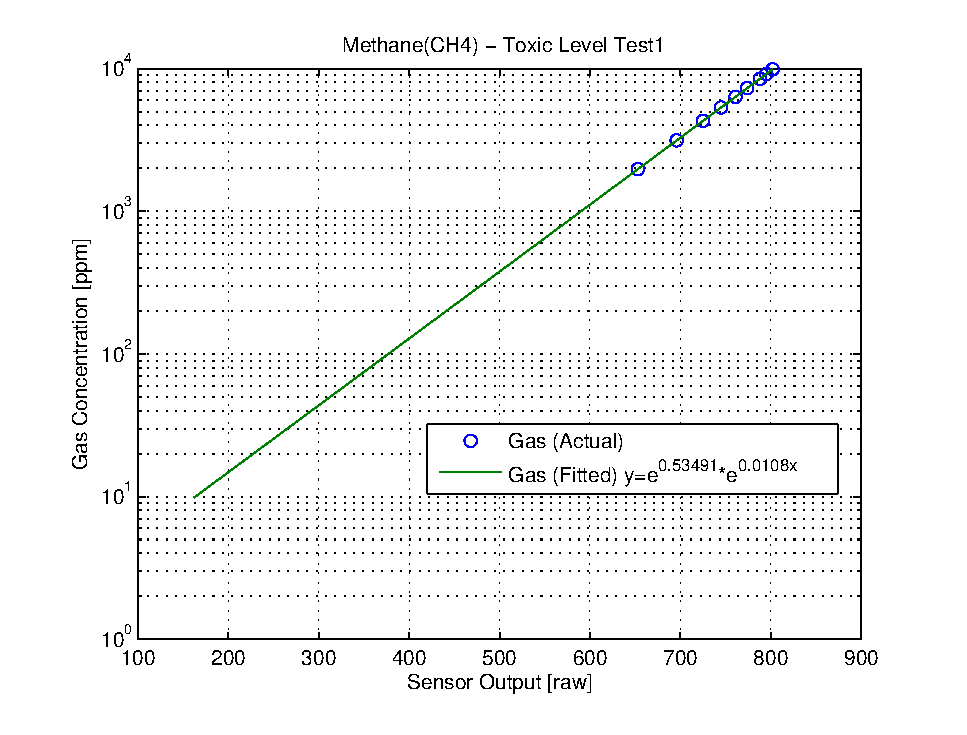
\includegraphics[width=0.4\textwidth]{./matlab/MethaneToxic.eps}
	\caption{Methane toxic levels. Threshold values are used to determine levels that are hazardous to humans.}
	\label{fig:methanetoxic}
\end{figure}

\begin{figure}
	\centering
	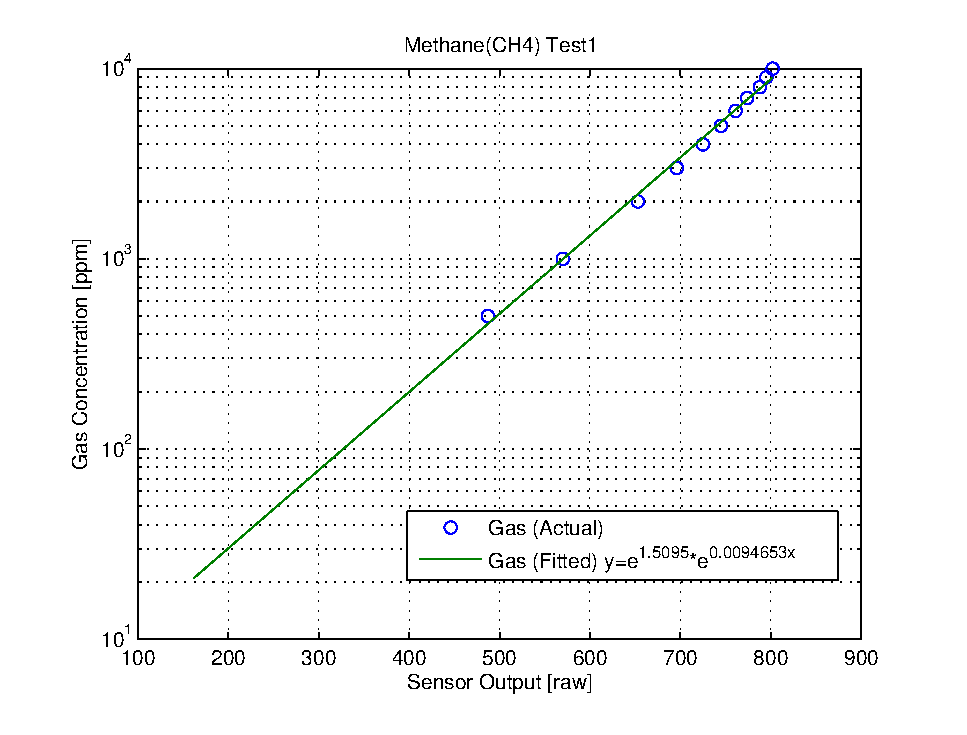
\includegraphics[width=0.4\textwidth]{./matlab/MethaneTest1.eps}
	\caption{Methane Gas test.}
	\label{fig:methanetest}
\end{figure}

\begin{figure}
	\centering
	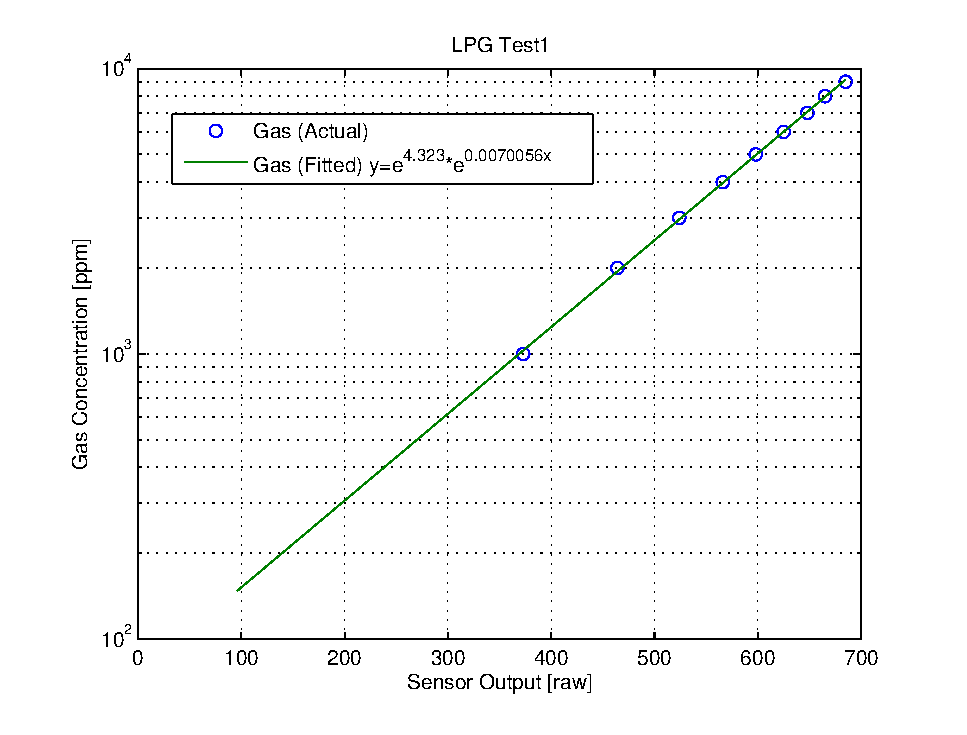
\includegraphics[width=0.4\textwidth]{./matlab/LPG.eps}
	\caption{Liquefied Petroleum Gas test.}
	\label{fig:lpg}
\end{figure}

\begin{figure}
	\centering
	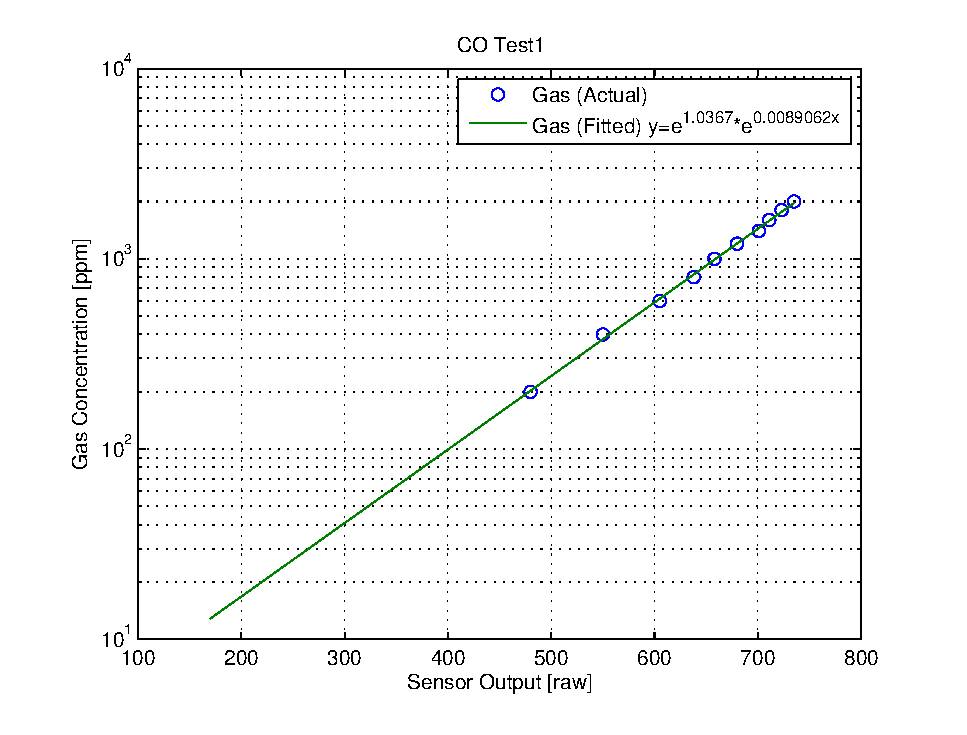
\includegraphics[width=0.4\textwidth]{./matlab/COTest1.eps}
	\caption{Carbon Monoxide test.}
	\label{fig:co}
\end{figure}

\begin{figure}
	\centering
	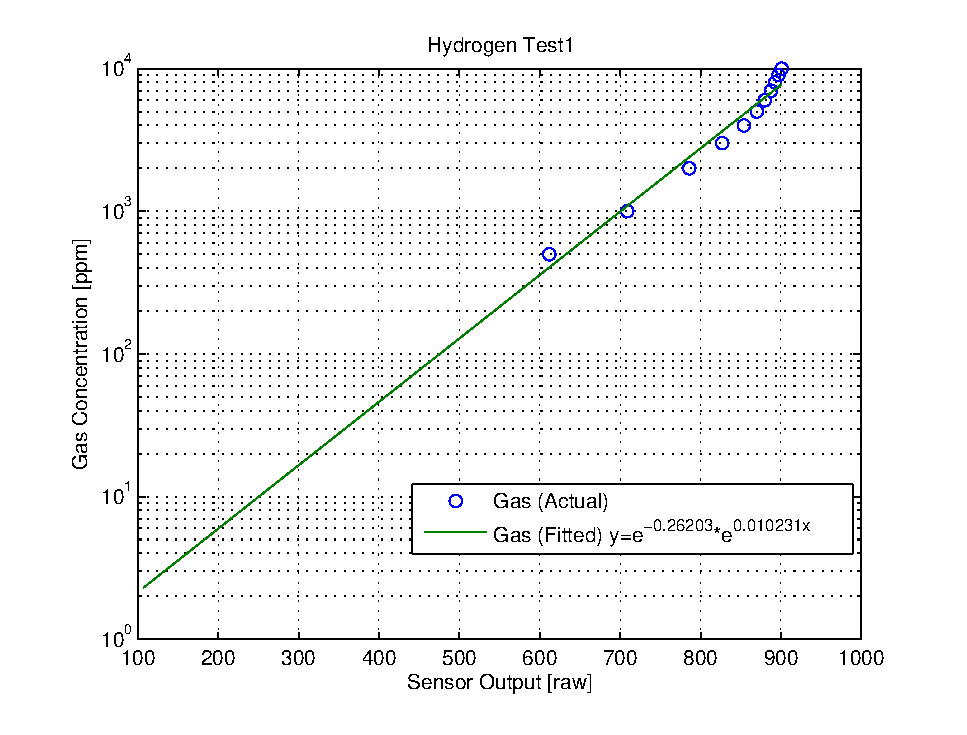
\includegraphics[width=0.4\textwidth]{./matlab/HydrogenTest1.eps}
	\caption{Hydrogen test.}
	\label{fig:hydrogen}
\end{figure}

Using the correction equations in software with the given sensor outputs, the final results closely match the expected concentrations. The corrected outputs will be able to discern the difference between a safe and a dangerous environment. 


%%%%%%%%%%%%%%%%%%%%%%%%%%%%%%%%%%%%%%%
% Conclusions
\section{Conclusions}\label{conclusions}
Industrial Hygiene monitoring and response functions possess the potential for improving efficiency and safety through the use of robots. Robotic systems such as the GVR-bot can remove humans from dangerous environments while accurately and reliably conducting tasks that are critical to operations on all Army installations. These improvements in efficiency and safety can be obtained in a fiscally responsible manner through the use of existing Army systems. Additionally, research conducted at the Academy benefits the Army long-term by exposing future officers to Army programs and technology at the beginning of their career.

%%%%%%%%%%%%%%%%%%%%%%%%%%%%%%%%%%%%%%%

%\addtolength{\textheight}{0cm}  % This command serves to balance the column lengths
                                  % on the last page of the document manually. It shortens
                                  % the textheight of the last page by a suitable amount.
                                  % This command does not take effect until the next page
                                  % so it should come on the page before the last. Make
                                  % sure that you do not shorten the textheight too much.

%%%%%%%%%%%%%%%%%%%%%%%%%%%%%%%%%%%%%%%

\bibliographystyle{bibliography/IEEEtran}
\bibliography{bibliography/IEEEabrv,bibliography/bibliography}

\end{document}
